\section{Experiments}
\label{experiments}

\subsection{Implementation Details}
\label{sec:implementation}

\subsubsection{Training details}
 Following recent works~\citep{zheng2025first,cheng2025reasoning,zheng2025parallelr1parallelthinkingreinforcement}, We employ Qwen2.5-3B~\cite{qwen2025qwen25technicalreport}, Qwen3-4B-Base and Qwen3-8B-Base~\cite{yang2025qwen3} as our backbone models. Following works~\citep{yu2025dapo,cheng2025reasoning,cui2025entropy}, we utilize the DAPO-Math-17K dataset~\citep{yu2025dapo} for training. Given its demonstrated stability and superiority over vanilla GRPO~\citep{yu2025dapo,cheng2025reasoning}, we adopt the DAPO algorithm~\cite{yu2025dapo} as both our baseline and the core optimization method for our \SDRL{} approach. 

We configure the learning rate at $1 \times 10^{-6}$ with a linear warm-up over the first 10 rollout steps. The rollout phase utilizes a prompt batch size of $256$, generating $8$ responses per prompt. For each debate pair, we generate $4$ responses for Qwen2.5-3B and $8$ responses for Qwen3-4B-Base and Qwen3-8B-Base. We utilize a sparse reward signal, assigning $+1$ for correct solutions and $-1$ otherwise. All training experiments are implemented within the verl framework~\citep{sheng2024hybridflow}. Additional configuration details are provided in the Appendix.

\subsubsection{Evaluation}

\textbf{Benchmarks.} Following prior work~\cite{choi2025debate,zhao2025majority,li2025off}, we conduct evaluations on the mathematical reasoning benchmarks MATH500~\citep{hendrycks2021measuring}, AMC 2023, and AIME 2024/2025.

\textbf{Multi-Agent Debate.} Consistent with established MAD literature~\citep{choi2025debate}, we primarily evaluate under the \textit{Decentralized MAD} setting~\cite{du2023improving,choi2025debate}, where each agent observes all peer responses from the previous round. Additional ablation studies on more debate frameworks are provided in Section~\ref{further_analysis}. We benchmark performance against the strong \textit{Majority Voting} baseline, which selects the most common answer from the initial round without debate. Our main experiments utilize $N=5$ agents and $T=1$ debate round; ablations on $N$ and $T$ are provided separately. Inference is conducted with a rollout temperature of $1.0$ and top-$p$ sampling ($p = 0.9$). For all MAD experiments, we report the average score across $5$ independent runs.

\textbf{Single-Agent Reasoning.} Following recent RL reasoning literature~\citep{guo2025deepseek,liu2025explore}, we also assess model performance without debate. For each prompt, we sample $K$ independent responses, and report the average accuracy ($mean@K$) and majority-vote accuracy ($maj@K$), setting $K=32$ for the AMC and AIME datasets, and $K=4$ for the MATH500 benchmarks. Further evaluation details are available in the Appendix.

\begin{table*}[t]
  \caption{Multi-agent debate performance comparison of different model architectures between the DAPO baseline and \SDRL{} across math reasoning benchmarks. The debate system contains $5$ agents. \textit{Maj} denotes the majority-vote accuracy of the agents' direct responses to the question. \textit{Debate} denotes the performance of the decentralized multi-agent system after debate round $1$. $\Delta$ is the difference between \textit{Maj} and \textit{Debate}. Best results are bolded.}
  \label{tab:main-multi}
  \begin{center}
    \resizebox{\textwidth}{!}{
      \begin{tabular}{lccccccccccccccc}
        \toprule
        Method
          & \multicolumn{3}{c}{MATH500}
          & \multicolumn{3}{c}{AMC23}
          & \multicolumn{3}{c}{AIME24}
          & \multicolumn{3}{c}{AIME25}
          & \multicolumn{3}{c}{Avg.} \\
        \cmidrule(lr){2-4}\cmidrule(lr){5-7}\cmidrule(lr){8-10}\cmidrule(lr){11-13}\cmidrule(lr){14-16}
          & Maj & Debate & $\Delta$
          & Maj & Debate & $\Delta$
          & Maj & Debate & $\Delta$
          & Maj & Debate & $\Delta$
          & Maj & Debate & $\Delta$ \\
        \midrule
        \multicolumn{16}{c}{Qwen2.5-3B} \\
        \midrule
        \emph{DAPO}               & 70.9 & 71.1 & 0.2  & 49.0 & 50.0 & 1.0  & 7.3 & 10.0 & 2.7  & 4.0 & 3.3 & -0.7 & 32.8 & 33.6 & 0.8 \\
        + \SDRL{}-rand        & 70.7 & 71.4 & \textbf{0.7}  & 49.2 & \textbf{53.8} & \textbf{4.6}  & 8.7 & 11.7 & 3.0  & \textbf{5.6} & \textbf{6.1} & 0.5  & 33.6 & \textbf{35.8} & \textbf{2.2} \\
        + \SDRL{}-freq         & \textbf{71.4} & \textbf{71.7} & 0.3  & \textbf{52.5} & 53.5 & 1.0  & \textbf{9.3} & \textbf{13.3} & \textbf{4.0}  & 3.3 & 4.7 & \textbf{1.4} & \textbf{34.1} & \textbf{35.8} & 1.7 \\
        \midrule
        \multicolumn{16}{c}{Qwen3-4B-Base} \\
        \midrule
        \emph{DAPO}               & 86.9 & 83.1 & -3.8 & \textbf{73.0} & 76.0 & 3.0 & 26.7 & 28.3 & 1.6 & 24.7 & 24.0 & -0.7 & 52.8 & 52.9 & 0.1 \\
        + \SDRL{}-rand        & \textbf{88.8} & \textbf{86.6} & -2.2 & 72.5 & \textbf{80.0} & \textbf{7.5} & \textbf{30.8} & 31.7 & 0.9 & 22.7 & 24.0 & \textbf{1.3} & 53.7 & 55.6 & 1.9 \\
        + \SDRL{}-freq         & 87.0 & 85.9 & \textbf{-1.1} & 72.5 & 79.0 & 6.5 & 28.7 & \textbf{36.0} & \textbf{7.3} & \textbf{28.7} & \textbf{30.0} & \textbf{1.3} & \textbf{54.2} & \textbf{57.7} & \textbf{3.5} \\
        \midrule
        \multicolumn{16}{c}{Qwen3-8B-Base} \\
        \midrule
        \emph{DAPO}               & 86.6 & 85.3 & -1.3 & 79.0 & 77.5 & -1.5 & 28.0 & 26.7 & -1.3 & 23.3 & 24.7 & 1.4 & 54.2 & 53.6 & -0.6 \\
        + \SDRL{}-rand     & 86.2 & 86.5 & \textbf{0.3} & \textbf{81.5} & 86.5 & 5.0 & 31.0 & 34.8 & 3.8 & \textbf{26.7} & 32.0 & 5.3 & 56.4 & 60.0 & 3.6 \\
        + \SDRL{}-freq     & \textbf{88.0} & \textbf{88.2} & 0.2 & 80.0 & \textbf{88.0} & \textbf{8.0} & \textbf{33.3} & \textbf{37.9} & \textbf{4.6} & 25.6 & \textbf{32.2} & \textbf{6.6} & \textbf{56.7} & \textbf{61.6} & \textbf{4.9} \\
        \bottomrule
      \end{tabular}
    }
  \end{center}
  \vskip -0.1in
\end{table*}


\subsection{Multi-Agent Debate}
\label{debate_exp}
Table~\ref{tab:main-multi} compares \SDRL{} with the DAPO baseline under the decentralized MAD setting with $N{=}5$ agents and one debate round. \SDRL{}-rand denotes random pairing, and \SDRL{}-freq denotes frequency-based pairing for debate pair construction. The main observation is that \SDRL{} consistently improves multi-agent debate across model architectures. The strongest results are achieved by \SDRL{}-freq, which gives the best average \textit{Debate} accuracy for Qwen3-4B-Base and Qwen3-8B-Base, and matches the best result for Qwen2.5-3B.

For Qwen2.5-3B, \SDRL{} improves the post-debate performance from $33.6$ to $35.8$ on average. \SDRL{}-rand gives the largest average debate gain, increasing $\Delta$ from $0.8$ to $2.2$. \SDRL{}-freq reaches the same best average \textit{Debate} accuracy of $35.8$ and gives the strongest AIME24 result, improving \textit{Debate} from $10.0$ to $13.3$ and $\Delta$ from $2.7$ to $4.0$. These results show that \SDRL{} makes even the smaller model more effective in decentralized debate.

The advantage of \SDRL{}-freq becomes clearer on stronger backbones. For Qwen3-4B-Base, \SDRL{}-freq improves the average \textit{Maj} accuracy from $52.8$ to $54.2$ and the average \textit{Debate} accuracy from $52.9$ to $57.7$. It also increases the average debate gain from $0.1$ to $3.5$. The largest improvement appears on AIME24, where \textit{Debate} increases from $28.3$ to $36.0$. For Qwen3-8B-Base, \SDRL{}-freq further strengthens this trend. It improves the average \textit{Maj} accuracy from $54.2$ to $56.7$, raises the average \textit{Debate} accuracy from $53.6$ to $61.6$, and increases the average debate gain to $\Delta=4.9$. It also achieves the best post-debate result on most benchmark for this backbone.

Overall, these results demonstrate that \SDRL{} trains reasoning LLMs to better participate in multi-agent debate. The improvement appears in both the quality of the initial response pool and the effectiveness of the debate step. Among the two pairing strategies, \SDRL{}-freq provides the most reliable gains, especially on stronger models and challenging benchmarks. This suggests that frequency-based pairing creates more informative debate contexts, allowing agents to better compare competing solutions, revise erroneous trajectories, and convert debate into consistent performance gains.

\begin{table*}[t]
  \caption{Single-agent performance comparison of different model architectures between the DAPO baseline and \SDRL{} across several math reasoning benchmarks.  We report the average accuracy $\mathrm{mean}@K$ and the majority-vote accuracy $\mathrm{maj}@K$ over $K$ independent runs. Best results are bolded.}
  \label{tab:main-single}
  \begin{center}
    \begin{small}
        \setlength{\tabcolsep}{4.5pt}
        \resizebox{\textwidth}{!}{%
        \begin{tabular}{lcccccccccc}
          \toprule
          Method
            & \multicolumn{2}{c}{MATH500}
            & \multicolumn{2}{c}{AMC23}
            & \multicolumn{2}{c}{AIME24}
            & \multicolumn{2}{c}{AIME25}
            & \multicolumn{2}{c}{Avg.} \\
          \cmidrule(lr){2-3}\cmidrule(lr){4-5}\cmidrule(lr){6-7}\cmidrule(lr){8-9}\cmidrule(lr){10-11}
            & mean@4 & maj@4
            & mean@32 & maj@32
            & mean@32 & maj@32
            & mean@32  & maj@32
            & mean & maj \\
          \midrule
          \multicolumn{11}{c}{Qwen2.5-3B} \\
          \midrule
          \emph{DAPO}      & 64.5 & 70.4 & 48.5 & 56.8 & 7.2 & 13.5 & 3.1 & 4.2 & 30.8 & 36.2 \\
          + \SDRL{}-rand      & 65.1 & 70.6 & 48.1 & 57.4 & \textbf{9.9} & 13.9 & \textbf{4.8} & \textbf{8.0} & 32.0 & \textbf{37.5} \\
          + \SDRL{}-freq       & \textbf{65.5} & \textbf{71.0} & \textbf{49.9} & \textbf{58.0} & 9.7 & \textbf{15.5} & 4.1 & 4.9 & \textbf{32.3} & 37.4 \\
          \midrule
          \multicolumn{11}{c}{Qwen3-4B-Base} \\
          \midrule
          \emph{DAPO}      & 82.9 & 84.4 & 71.9 & 81.4 & 24.8 & 31.1 & 24.9 & 27.8 & 51.1 & 56.2 \\
          + \SDRL{}-rand      & \textbf{83.7} & 85.8 & 72.3 & \textbf{84.1} & 25.9 & \textbf{35.1} & 20.4 & 27.6 & 50.6 & 58.2 \\
          + \SDRL{}-freq       & 82.2 & \textbf{86.2} & \textbf{74.2} & 83.0 & \textbf{26.6} & 34.4 & \textbf{26.6} & \textbf{37.2} & \textbf{52.4} & \textbf{60.2} \\
          \midrule
          \multicolumn{11}{c}{Qwen3-8B-Base} \\
          \midrule
          \emph{DAPO}      & 83.2 & 85.4 & 77.7 & 86.8 & 26.1 & 33.0 & 23.6 & 26.6 & 52.7 & 58.0 \\
          + \SDRL{}-rand   & 83.4 & 86.6 & 78.3 & 90.5 & 30.1 & 38.4 & \textbf{27.3} & \textbf{35.8} & 54.8 & 62.8 \\
          + \SDRL{}-freq   & \textbf{85.4} & \textbf{88.4} & \textbf{80.6} & \textbf{93.6} & \textbf{32.6} & \textbf{43.4} & 26.6 & 34.4 & \textbf{56.3} & \textbf{65.0} \\
          \bottomrule
        \end{tabular}
        }
    \end{small}
  \end{center}
  \vskip -0.1in
\end{table*}

\subsection{Single-Agent Reasoning}
\label{single_exp}

We follow prior reasoning LLM evaluation protocols~\cite{yu2025dapo} and evaluate each model as a single agent. Table~\ref{tab:main-single} reports both $\mathrm{mean}@K$ and $\mathrm{maj}@K$ across benchmarks. Overall, \SDRL{} improves single-agent reasoning across all three model architectures. This shows that training with \SDRL{} not only prepares models for debate, but also strengthens standalone problem-solving ability.

For Qwen2.5-3B, \SDRL{}-rand increases the average $\mathrm{mean}@K$ from $30.8$ to $32.0$ and the average $\mathrm{maj}@K$ from $36.2$ to $37.5$. \SDRL{}-freq further improves the average $\mathrm{mean}@K$ to $32.3$ and reaches a comparable average $\mathrm{maj}@K$ of $37.4$. For Qwen3-4B-Base, \SDRL{}-freq gives the strongest overall results, improving the average $\mathrm{mean}@K$ from $51.1$ to $52.4$ and the average $\mathrm{maj}@K$ from $56.2$ to $60.2$.
The advantage of \SDRL{}-freq becomes more pronounced on Qwen3-8B-Base. It improves the average $\mathrm{mean}@K$ from $52.7$ to $56.3$ and the average $\mathrm{maj}@K$ from $58.0$ to $65.0$, achieving the best average result among all methods. It also obtains the best performance on MATH500, AMC23, and AIME24. In particular, AIME24 $\mathrm{maj}@32$ improves from $33.0$ to $43.4$, and AMC23 $\mathrm{maj}@32$ improves from $86.8$ to $93.6$.

Overall, the single-agent results demonstrate that \SDRL{} improves reasoning LLMs beyond the multi-agent setting. By jointly optimizing initial and debate-conditioned responses, \SDRL{} improves the quality of direct responses while preserving the capabilities needed for effective debate. Among the two pairing strategies, \SDRL{}-freq provides the strongest overall performance, suggesting that frequency-based debate construction also benefits standalone reasoning.

% ==============================================================================
\subsection{Further Analysis}
\label{further_analysis}
As \SDRL{} with frequency-based pairing yields better overall performance than random pairing, we conduct additional experiments using \SDRL{}+freq. More experiments, including the measurement of private critique $\delta$, can be found in Appendix.

% ==================================
% Number of rounds
% ==================================
\textbf{Debate Rounds.} We evaluate more debate rounds in the decentralized MAD setting with $5$ agents, and report the results in Figure~\ref{fig:round}. Compared with the DAPO baseline, \SDRL{} achieves higher accuracy across all debate rounds. Moreover, \SDRL{} typically yields larger improvements as the number of rounds increases. Except for MATH500, the debate performance of both DAPO and \SDRL{} increases in the early rounds and then declines, which is consistent with our theoretical analysis that debate improves in
early rounds but peaks quickly and can decline later. More analysis on MATH500 can be found in the Appendix.

\begin{figure*}[!t]
  \begin{center}
    \centerline{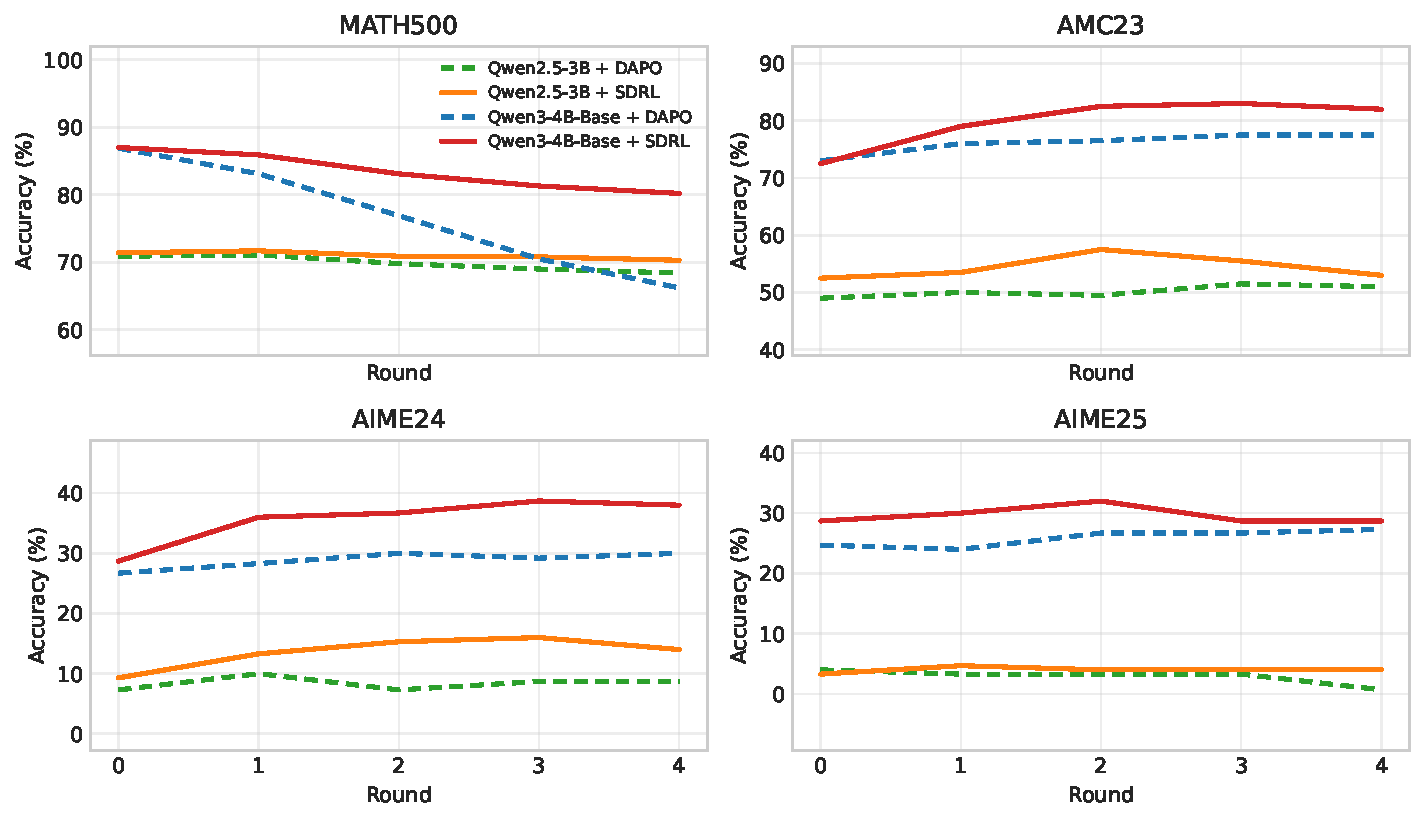
\includegraphics[width=0.8\textwidth]{fig/round-ablation.pdf}}
    \caption{
      Debate performance of $5$ agents in different debate rounds under the decentralized MAD setting.
    }
    \label{fig:round}
  \end{center}
  \vspace{-25pt}
\end{figure*}

% =========================
% Table 2: Number of agents
% =========================
\textbf{Number of Agents.} We report experimental results for the decentralized MAD system with varying numbers of agents under a single debate round, as shown in Table~\ref{tab:num_agents}. Overall, \SDRL{} consistently outperforms the DAPO baseline across all agent settings. Increasing the number of agents from $3$ to $5$ leads to consistent improvements in average debate performance. However, in the $7$-agent setting on AMC23, AIME24, and AIME25, performance drops because we reduce the max response tokens during generation to keep the debate sequence within the model context window, which results in truncated and incomplete responses.

\textbf{Additional Debate Frameworks.} Following~\cite{choi2025debate}, we evaluate \SDRL{} under additional debate frameworks. These include Sparse MAD~\cite{li2024improving}, a variant of decentralized MAD that uses a sparse communication topology to improve efficiency, and Centralized MAD~\cite{guo2024large}, where a central agent aggregates peers' responses and produces an updated response at each round. The results are reported in Table~\ref{tab:debate-framework}. Overall, \SDRL{} outperforms the DAPO baseline in both debate accuracy and the improvement brought by debate across all settings, demonstrating the robustness of \SDRL{}-trained models under different debate frameworks.

\begin{table*}[!t]
  \caption{Ablation on the number of agents $N$ in decentralized MAD setting. \textit{Maj} denotes the majority-vote accuracy of the agents' direct responses to the question. \textit{Debate} denotes the performance of the decentralized multi-agent system after debate round $1$. $\Delta$ is the difference between \textit{Maj} and \textit{Debate}.}
  \label{tab:num_agents}
  \begin{center}
    \resizebox{\textwidth}{!}{%
      \begin{tabular}{lccccccccccccccc}
        \toprule
        Method
          & \multicolumn{3}{c}{MATH500}
          & \multicolumn{3}{c}{AMC23}
          & \multicolumn{3}{c}{AIME24}
          & \multicolumn{3}{c}{AIME25}
          & \multicolumn{3}{c}{Avg.} \\
        \cmidrule(lr){2-4}\cmidrule(lr){5-7}\cmidrule(lr){8-10}\cmidrule(lr){11-13}\cmidrule(lr){14-16}
          & Maj & Debate & $\Delta$
          & Maj & Debate & $\Delta$
          & Maj & Debate & $\Delta$
          & Maj & Debate & $\Delta$
          & Maj & Debate & $\Delta$ \\
        \midrule
        \multicolumn{16}{c}{\textbf{Qwen2.5-3B}} \\
        \midrule
        DAPO (N=3) & 67.5 & 68.2 & 0.7  & 48.0 & 50.0 & 2.0 & 4.0 & 6.7 & 2.7 & 1.3 & 1.3 & 0.0 & 30.2 & 31.6 & 1.4 \\
        % DAPO (N=4) & -- & -- & -- & 46.0 & 44.5 & -1.5 & 4.0 & 9.3 & +5.3 & 2.7 & 2.7 & +0.0 & 29.7 & 30.8 & +1.1 \\
        DAPO (N=5) & 70.9 & 71.1 & 0.2  & 49.0 & 50.0 & 1.0  & 7.3 & 10.0 & 2.7  & 4.0 & 3.3 & -0.7 & 32.8 & 33.6 & 0.8 \\
        % DAPO (N=6) & -- & -- & -- & 45.0 & 48.5 & +3.5 & 7.3 & 8.7 & +1.3 & 2.7 & 2.7 & +0.0 & 30.8 & 32.1 & +1.3 \\
        DAPO (N=7) & 72.4 & 71.9 & -0.5 & 49.0 & 51.0 & 2.0 & 6.7 & 9.3 & 2.7 & 3.3 & 2.7 & -0.7 & 32.9 & 33.7 & 0.9 \\
        +\SDRL{} (N=3) & 66.2 & 67.3 & 1.1  & 51.0 & 55.0 & 4.0 & 11.3 & 13.3 & 2.0 & 1.3 & 4.7 & 3.3 & 32.5 & 35.1 & 2.6 \\
        % +\SDRL{} (N=4) & -- & -- & -- & 52.5 & 58.0 & +5.5 & 6.7 & 10.7 & +4.0 & 6.7 & 4.7 & -2.0 & 33.0 & 35.4 & +2.4 \\
        +\SDRL{} (N=5) & 71.4 & 71.7 & 0.3  & 52.5 & 53.5 & 1.0  & 9.3 & 13.3 & 4.0  & 3.3 & 4.7 & 1.4  & 34.1 & 35.8 & 1.7 \\
        % +\SDRL{} (N=6) & -- & -- & -- & 51.5 & 57.5 & +6.0 & 12.7 & 13.3 & +0.7 & 6.0 & 4.0 & -2.0 & 34.6 & 35.8 & +1.2 \\
        +\SDRL{} (N=7) & 71.5 & 71.9 & 0.4  & 53.0 & 55.0 & 2.0 & 12.0 & 14.7 & 2.7 & 4.7 & 6.0 & 1.3 & 35.3 & 36.9 & 1.6 \\
        \midrule
        \multicolumn{16}{c}{\textbf{Qwen3-4B-Base}} \\
        \midrule
        DAPO (N=3) & 85.2 & 82.8 & -2.4 & 68.0 & 70.5 & 2.5 & 20.7 & 25.3 & 4.7 & 24.7 & 23.3 & -1.3 & 49.6 & 50.5 & 0.9 \\
        % DAPO (N=4)                  & -- & -- & -- & -- & -- & -- & -- & -- & -- & -- & -- & -- & -- & -- & -- \\
        DAPO (N=5)    & 86.9 & 83.1 & -3.8 & 73.0 & 76.0 & 3.0 & 26.7 & 28.3 & 1.6 & 24.7 & 24.0 & -0.7 & 52.8 & 52.9 & 0.1 \\
        % DAPO (N=6)                  & -- & -- & -- & -- & -- & -- & -- & -- & -- & -- & -- & -- & -- & -- & -- \\
        DAPO (N=7) & 87.7 & 84.0 & -3.7 & 72.0 & 76.0 & 4.0 & 23.3 & 26.0 & 2.7 & 23.3 & 24.7 & 1.3 & 51.6 & 52.7 & 1.1 \\
        +\SDRL{} (N=3) & 84.4 & 83.6 & -0.7 & 70.0 & 76.7 & 6.7 & 24.7 & 34.0 & 9.3 & 20.0 & 23.3 & 3.3 & 49.8 & 54.4 & 4.7 \\
        % +\SDRL{} (N=4)          & -- & -- & -- & -- & -- & -- & -- & -- & -- & -- & -- & -- & -- & -- & -- \\
        +\SDRL{} (N=5)    & 87.0 & 85.9 & -1.1 & 72.5 & 79.0 & 6.5 & 28.7 & 36.0 & 7.3 & 28.7 & 30.0 & 1.3 & 54.2 & 57.7 & 3.5 \\
        % +\SDRL{} (N=6)          & -- & -- & -- & -- & -- & -- & -- & -- & -- & -- & -- & -- & -- & -- & -- \\
        +\SDRL{} (N=7) & 88.1 & 85.9 & -2.2 & 70.0 & 81.7 & 11.7 & 23.3 & 32.0 & 8.7 & 22.7 & 28.7 & 6.0 & 51.0 & 57.1 & 6.1 \\
        \bottomrule
      \end{tabular}%
    }
  \end{center}
  \vskip -0.1in
\end{table*}


\begin{table*}[t]
  \caption{Multi-agent debate performance under different debate settings. The debate system contains $5$ agents. \textit{Maj} denotes the majority-vote accuracy of the agents' direct responses to the question. \textit{Debate} denotes the performance of the decentralized multi-agent system after debate round $1$. $\Delta$ is the difference between \textit{Maj} and \textit{Debate}.}
  \label{tab:debate-framework}
  \begin{center}
    \resizebox{\textwidth}{!}{
      \begin{tabular}{lccccccccccccccc}
        \toprule
        Method
          & \multicolumn{3}{c}{MATH500}
          & \multicolumn{3}{c}{AMC23}
          & \multicolumn{3}{c}{AIME24}
          & \multicolumn{3}{c}{AIME25}
          & \multicolumn{3}{c}{Avg.} \\
        \cmidrule(lr){2-4}\cmidrule(lr){5-7}\cmidrule(lr){8-10}\cmidrule(lr){11-13}\cmidrule(lr){14-16}
          & Maj & Debate & $\Delta$
          & Maj & Debate & $\Delta$
          & Maj & Debate & $\Delta$
          & Maj & Debate & $\Delta$
          & Maj & Debate & $\Delta$ \\
        \midrule
        \multicolumn{16}{c}{\textbf{Qwen2.5-3B}} \\
        \midrule
        DAPO (sparse)              & 71.4 & 70.8 & -0.6 & 47.5 & 44.2 & -3.3 & 10.0 & 6.7 & -3.3 & 3.3 & 3.3 & 0.0 & 33.1 & 31.3 & -1.8 \\
        DAPO (centralized)          & 62.5 & 63.2 & 0.7  & 38.3 & 42.5 & 4.2  & 6.7  & 4.4 & -2.2 & 3.3 & 5.6 & 2.2  & 27.7 & 28.9 & 1.2 \\
        +\SDRL{} (sparse)      & 70.5 & 71.0 & 0.5  & 48.3 & 52.5 & 4.2  & 6.7  & 8.9 & 2.2  & 4.4 & 4.4 & 0.0  & 32.5 & 34.2 & 1.7 \\
        +\SDRL{} (centralized)  & 64.5 & 65.5 & 1.0  & 45.0 & 52.5 & 7.5  & 4.4  & 10.0 & 5.6 & 4.4 & 8.9 & 4.4  & 29.6 & 34.2 & 4.6 \\
        \midrule
        \multicolumn{16}{c}{\textbf{Qwen3-4B-Base}} \\
        \midrule
        DAPO (sparse)              & 86.5 & 86.0 & -0.6 & 70.5 & 78.0 & 7.5 & 22.7 & 24.7 & 2.0 & 24.0 & 25.3 & 1.3 & 50.9 & 53.5 & 2.6 \\
        DAPO (centralized)          & 80.7 & 79.5 & -1.2 & 64.0 & 72.0 & 8.0 & 23.3 & 27.3 & 4.0 & 21.4 & 22.0 & 0.6 & 47.4 & 50.2 & 2.9 \\
        +\SDRL{} (sparse)      & 86.7 & 86.6 & -0.1 & 69.5 & 78.5 & 9.0 & 28.7 & 36.0 & 7.3 & 28.7 & 33.3 & 4.6 & 53.4 & 58.6 & 5.2 \\
        +\SDRL{} (centralized)  & 80.5 & 81.0 & 0.5  & 66.5 & 78.0 & 11.5 & 25.3 & 34.0 & 8.7 & 25.3 & 26.7 & 1.4 & 49.4 & 54.9 & 5.5 \\
        \bottomrule
      \end{tabular}
    }
  \end{center}
  \vskip -0.1in
\end{table*}